% Este arquivo .tex será incluído no arquivo .tex principal. Não é preciso
% declarar nenhum cabeçalho

\section{CACo -- Centro Acadêmico da Computação}

\begin{figure}[H]
    \centering
    
\includegraphics[scale=0.37]{img/caco/logo.png}
\end{figure}

Bixo, o CACo é o seu centro acadêmico. Um CA é uma entidade estudantil que, em
linhas gerais, deve trabalhar para garantir os interesses dos estudantes e
melhorar o curso e a faculdade a que pertence. O CACo é formado pelos alunos de
graduação tanto em Engenharia quanto em Ciência da Computação da Unicamp, bem
como os alunos de pós-graduação do IC. Todo e qualquer aluno desses cursos é
membro do CACo e isso inclui você.

Um centro acadêmico é parte do famoso ``movimento estudantil'' de que você
provavelmente já ouviu falar. Mas não se engane! Pergunte para o seu pai o que
ele pensa quando lê ``movimento estudantil'' e ele vai dizer que vê um bando de
estudantes desocupados associados a um partido político de esquerda que saem por
aí protestando contra o sistema e queimando ônibus pelas ruas. Se você pensa
assim, mude sua ideia: o CACo não é nada disso.

\begin{figure}[H]
    \centering
    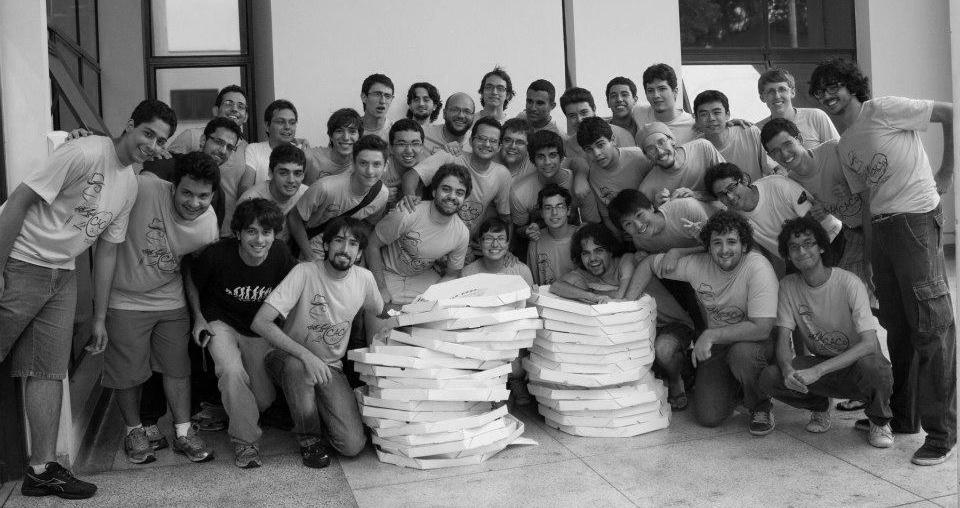
\includegraphics[scale=0.22]{img/caco/pizzada.jpg}
\end{figure}

O CACo tem como função representar os estudantes no âmbito acadêmico, ou seja,
perante o IC, a FEEC e a Unicamp. Mas o que o CACo faz? De forma simplificada,
procuramos ser porta-voz dos alunos. Reivindicamos espaço físico decente para os
alunos, alteração nas matérias e professores, promovemos discussões sobre temas
polêmicos e delicados, dentre muitas outras atividades.

Quer um exemplo? Esse estupendo manual que você está lendo neste exato momento
foi confeccionado pelo seu centro acadêmico para lhe ajudar no início da sua
vida universitária e, na verdade, você ainda vai se pegar recorrendo ao seu
Manual várias vezes durante seus quatro, cinco, doze anos na Unicamp.

Uma grande função do CACo é prezar pela qualidade dos cursos e fazemos isso, por
exemplo, através de discussões com o próprio Instituto, onde levamos reclamações
e reivindicações dos alunos para os coordenadores e professores.

\begin{figure}[H]
    \centering
    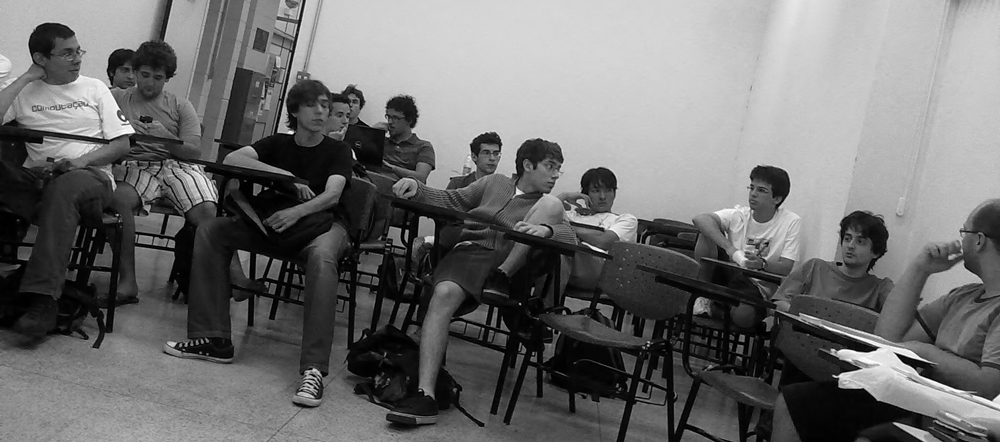
\includegraphics[scale=0.21]{img/caco/reuniao.jpg}
\end{figure}

Uma outra função do CACo é integrar os estudantes de computação da Unicamp. Para
isso, realizamos diversos eventos como o CineCACo, o PipoCACo, o CACo Games, o
CACo Series of Poker e a grande comemoração do Aniversário do CACo, que contou
com pizza de graça para mais de duzentos alunos! Tentamos também facilitar a
vida da galera através dos armários que alugamos, o Banco de Livros, o Banco de
Provas (o maior da Unicamp) e a máquina de café que colocamos no IC.

Repetindo o que foi dito antes: bixo, o CACo é o \textbf{seu} Centro Acadêmico.
Tudo que dissemos que fazemos pelos alunos, queremos fazer por você também. Por
isso, quando houver algum problema envolvendo a FEEC, o IC, os professores ou
qualquer coisa do tipo, não hesite em nos procurar. O CACo sempre lhe dará todo
o suporte necessário. Se tiver reclamação ou sugestão relacionada ao próprio
CACo, também estaremos aqui para ouvir. Mais do que isso, venha participar de
uma de nossas reuniões, que são abertas a você e todos os alunos de computação
da Unicamp.

\begin{figure}[H]
    \centering
    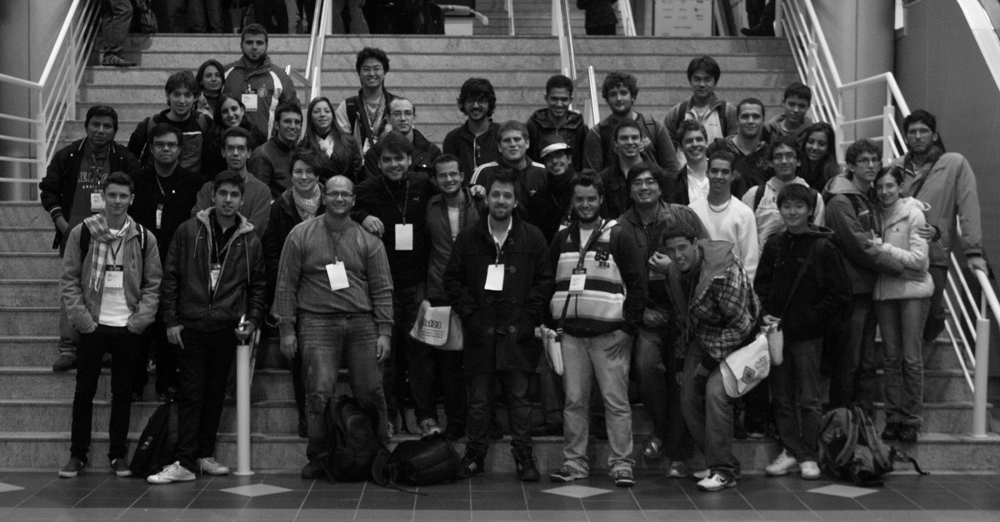
\includegraphics[scale=0.21]{img/caco/fisl2.jpg}
\end{figure}

Participar do CACo é uma experiência diferente de tudo aquilo que você terá na
sua graduação. É a chance de aprender e crescer de uma forma que não acontece em
nenhuma aula de cálculo. É uma oportunidade de conhecer seus veteranos e também
seus amiguinhos bixos. Mas, acima de tudo, é uma experiência pessoal onde você
vai aprender a se expressar, argumentar, defender suas ideias, falar em público
e pensar no coletivo. Você entrará em contato com muita gente que provavelmente
você nunca iria conhecer e, com certeza, fará amizade com muitos deles. Por
esses e muitos outros motivos é que você, bixo, deve vir a pelo menos uma
reunião do CACo e sentir na pele tudo o que foi dito aqui. Venha nos ajudar a
fortalecer ainda mais o melhor CA da Unicamp. Até a reunião!

\begin{compactitemize}
    \item  E-mail: \email{caco@ic.unicamp.br}
    \item  Site: \url{www.caco.ic.unicamp.br}
    \item  Reuniões: você será informado no começo do semestre sobre os horários das reuniões. Participe!
\end{compactitemize}

Veja a seguir algumas das atividades que o CACo pratica:

\subsection{Avaliação de Curso e Reforma Curricular}

Uma vez por semestre, ocorre a reunião de avaliação de curso da qual participam
alunos, coordenadores e professores, além de responsáveis pela infraestrutura do
IC e da FEEC. Nela, são discutidos problemas relativos aos cursos, que vão desde
professores ruins até cadeiras quebradas. São avaliadas as disciplinas,
apontados problemas e indicadas soluções. A participação dos alunos é muito
importante, afinal somos nós que mais ganhamos e perdemos com o bom e o ruim de
nossos cursos. Por isso, o CACo participa dessa reunião levando a opinião dos
alunos para serem debatidas.

A avaliação de curso também visa a reforma curricular dos cursos. O catálogo do
curso (disciplinas que devem ser cursadas) é alterado todos os anos e a reunião
de avaliação tem grande papel nessas alterações.

\subsection{Caravana para o fisl}

O CACo organiza anualmente uma caravana para o fisl, o Fórum Internacional de
Software Livre, que acontece em Porto Alegre. O fisl reúne milhares de pessoas
de todo o mundo e conta com palestras e profissionais de renome. O Fórum é um
ótimo modo de entrar em contato com o mundo da computação e a caravana é uma
ótima e barata maneira de ir e tembém de socializar com outros computeiros.

\begin{figure}[H]
    \centering
    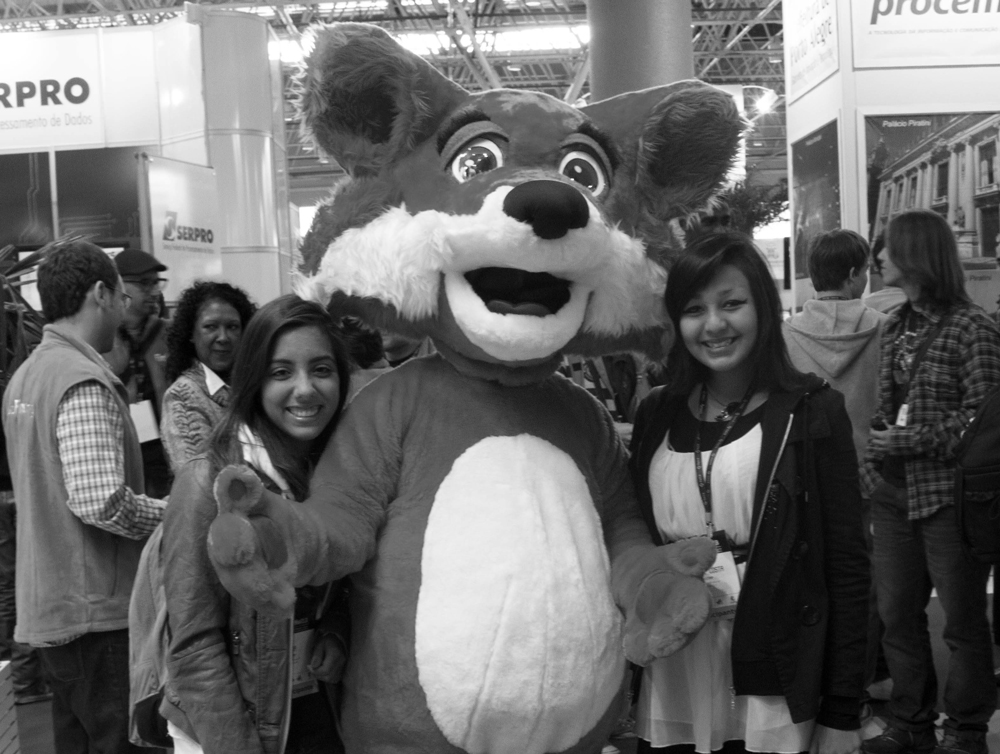
\includegraphics[scale=0.21]{img/caco/fisl.jpg}
\end{figure}

\subsection{Pesquisa Salarial}

Em 2010, com a colaboração do diretor do IC, o professor Hans Liesenberg, e da
rede social Reunion, promovemos uma pesquisa salarial com ex-alunos de
computação, que ajudou a fornecer um bom panorama da realidade em que se
encontra o profissional formado pela Unicamp na área de computação. A pesquisa
está disponível no site do CACo.

\subsection{CineCACo}

Por que não juntar com a galera no IC para assistir um filme com pipoca e
refriegerante de graça?

\subsection{PipoCACo}

Os PipoCACos são eventos de discussão sobre assuntos polêmicos, mas sem
comentários sobre  mamilos. Trata-se de um espaço para que toda a Computação
possa discutir um assunto de interesse geral. Por exemplo, já realizamos
PipoCACos sobre cotas em universidades públicas, sobre o Enade e semestralmente
fazemos o PipoCACo de Avaliação de Curso, onde reunimos as reclamações dos
alunos para a reunião de avaliação. Além de um ótimo local para ouvir opiniões e
debater, os PipoCACos são regados a refrigerante e pipoca por nossa conta!

\subsection{Palestra Azoide/Bzoide}

Chega um momento na vida de todo computeiro engenheiro em que ele deve responder
às questões fundamentais como: De onde viemos? Para onde vamos? Onde vamos
almoçar hoje? Vou ser Azoide ou Bzoide?

O curso de Engenharia de Computação da Unicamp se divide em duas habilitações,
também conhecidas como modalidades: AA e AB. A diferença? Não é simples! Por
isso, o CACo organiza uma série de palestras a fim de ajudá-lo a escolher a
modalidade que mais lhe agrada.

\subsection{CACo Series of Poker}

O lendário torneio de Poker do CACo. Aberto a toda a computação, o CSoP é um
ótimo evento de integração e já contou com cinco edições de absoluto sucesso!
Você será informado da data do próximo, fique ligado!

\begin{figure}[H]
    \centering
    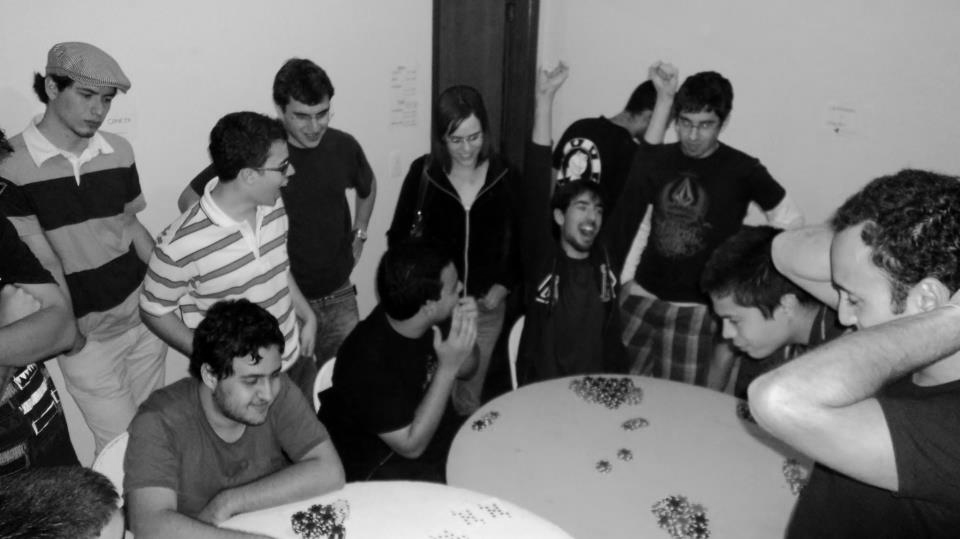
\includegraphics[scale=0.21]{img/caco/poker2.jpg}
\end{figure}

\subsection{Salinha}

A sede do CACo fica na nossa salinha no IC-3. Munida de uma incrível mesa de
sinuca, ela está aberta 24/7 para todos os computeiros que queiram jogar.

\subsection{Atendimento}

O CACo realiza atendimentos na nossa salinha. Nesses horários, você poderá
comprar nossos produtos, se inscrever em algum de nossos eventos ou só bater
papo com a gente mesmo. Os horários de atendimento serão divulgados no início do
semestre e você pode conferi-los no site do CACo.

\begin{figure}[H]
    \centering
    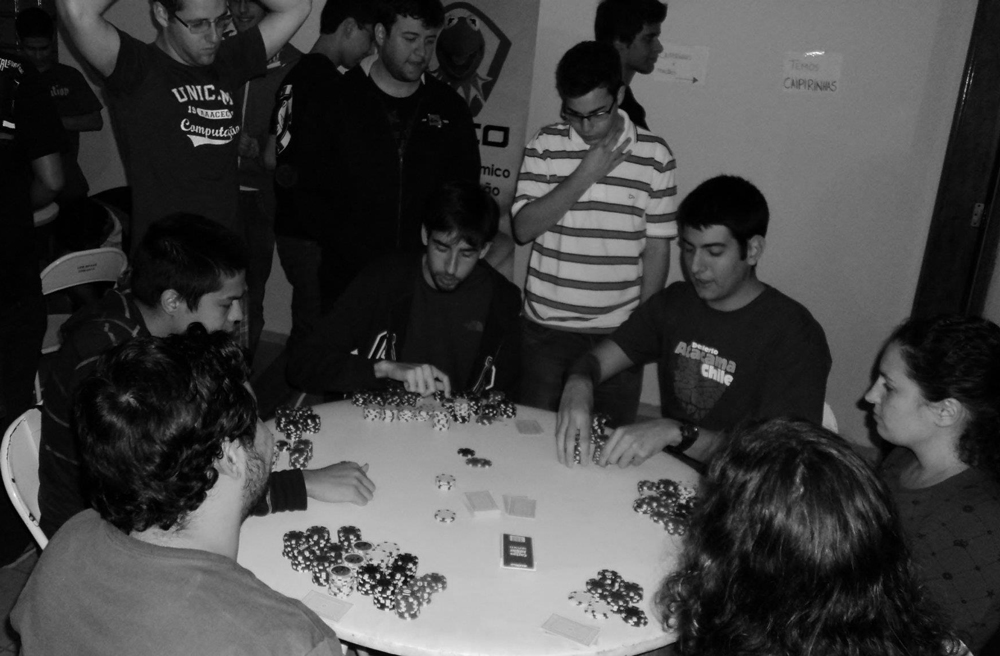
\includegraphics[scale=0.21]{img/caco/poker.jpg}
\end{figure}

\subsection{Gestão}

O CACo tem uma gestão composta de gente bonita e charmosa. Não se preocupe, se
você não é bonito nem charmoso, você ainda pode entrar na gestão... talvez. A
atual gestão foi eleita em novembro de 2012 e deve permanecer até outubro de
2013. Mas não pense que só a gestão gere o CACo. Mais uma vez: o CACo é o seu
centro acadêmico. Você e toda a computação também fazem parte do CACo e têm
papel nas nossas decisões e discussões.

Para ficar mais integrado ao que ocorre no seu centro acadêmico, como suas
ações, projetos e quais os problemas atuais, você pode se increver na lista do
CACo no Google Groups por meio do link:
\url{groups.google.com/group/cacounicamp}.

\begin{figure}[H]
    \centering
    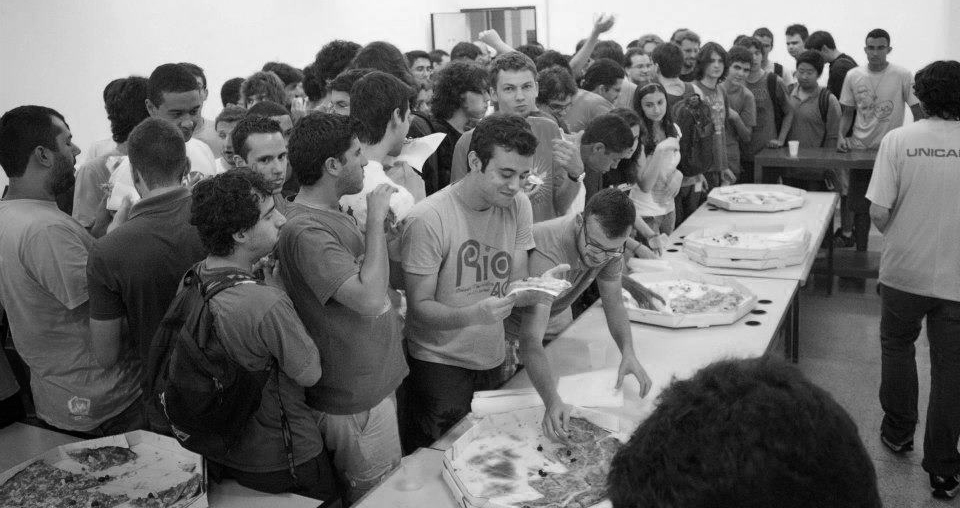
\includegraphics[scale=0.21]{img/caco/pizzada2.jpg}
\end{figure}

\begin{figure}[H]
    \centering
    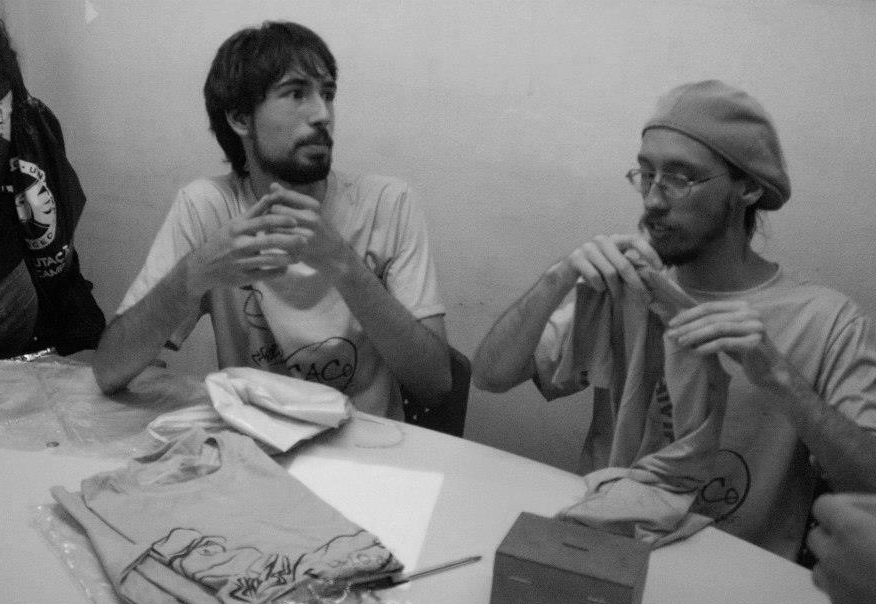
\includegraphics[scale=0.24]{img/caco/eleicao.jpg}
\end{figure}

\subsubsection*{Chapa ``CACoCota'' (2012/2013)}

\begin{itemize}
    \item   \textbf{Presidência}
        \\Julia Ramos Beltrão (Julia EC011)

    \item   \textbf{Coordenadoria Administrativa}
        \\Alexandre Novais de Medeiros (Salsicha CC011)
        \\Victor Rodrigues Matsuguma (Preciso EC011)

    \item   \textbf{Coodenadoria Financeira}
        \\Gabriel Militão Vinhas Lopes (Gagau EC012)
        \\André Felipe Barros Selva (Selva EC09)
        \\Guilherme Bueno Andrade (Laika EC012)

    \item   \textbf{Coordenadoria de Ensino e Graduação}
        \\Pedro Henrique Azevedo Amorim (Amorim EC011)
        \\Brunno Rodrigues Arangues (Brunno EC010)

    \item   \textbf{Coordenadoria de Ensino e Pós-Graduação}
        \\Eric Velten de Melo (Eric EC07)

    \item   \textbf{Coordenadoria de Comunicação}
        \\Pedro Cordeiro de Almeida (Pedroka CC012)
        \\Yuri Corrêa Pinto Soares (Yuri CC012)
        \\Gérson de Paulo Carlos (Gérson EC09)

    \item   \textbf{Coordenadoria de Eventos e Cultura}
        \\Antonio José Pinheiro Prado (Alegria EC012)
        \\Murilo Vieira Santa Bárbara (Buxexa EC012)
        \\Wesley Marques Dias (Kiabbo EC010)
        \\Humberto Aboud Torres Lobo (Sheldon EC010)
        \\Gustavo Menezes Rocha (Espanhol EC011)
        \\William Hideki Azana Tustumi (William EC011)

    \item   \textbf{Coordenadoria de Marketing}
        \\Matheus Jun Ota (Ota CC012)
        \\Gabriel Rolfsen Franzoni (Clits EC012)
        \\Thiago Rosario Caetano (Thiago EC010)
        \\Jucélio Evangelista Fonseca (Jeff CC012)

    \item   \textbf{Coordenadoria de Produtos}
        \\Hugo Aboud Torres Lobo (Hugo EC012)
        \\José Américo Nabuco Leva Ferreira de Freitas (Jota EC010)

    \item   \textbf{Coordenadoria Tecnológica}
        \\Gabriel Hidasy Rezende (Sam EC011)
        \\Gustavo de Mello Crivelli (Jobs EC012)
        \\Matheus Mostiack Pomaleski (Poma EC011)
        \\Pedro Emílio Machado de Brito (Asmina EC012)
\end{itemize}

As gestões dos anos anteriores podem ser vistas no site do CACo.

\begin{figure}[H]
    \centering
    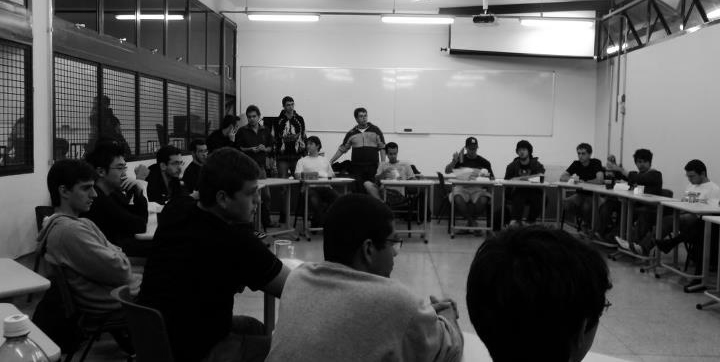
\includegraphics[scale=0.29]{img/caco/pipocaco.jpg}
\end{figure}
